\باب{ماورائی تفاعل}
        ریاضیات میں بہت سے تفاعل ایک دوسرے کے الٹ ہیں۔ غالباً سب سے زیادہ جانی پہچانی الٹ تفاعل کی جوڑی \عددی{\ln x} اور \عددی{e^x} ہے۔ موزوں وقفہ پر پابند تکونیاتی تفاعل کے اہم الٹ پائے  جاتے ہیں۔ اسی طرح  لوگارتھمی اور قوت نمائی تفاعل کے دیگر الٹ جوڑیاں پائی جاتی ہیں۔ ہذلولی تفاعل اور ان کے الٹ تفاعل کا استعمال آویزاں رسی، منتقلی حرکی توانائی، اور ہوا میں گرتے ہوئے جسم پر قوت رگڑ کے مسائل میں کام آتے ہیں۔ اس باب میں ان تمام تفاعل پر غور کیا جائے گا۔ ان مسئلوں کا بھی ذکر کیا جائے گا جنہیں یہ تفاعل حل کرنے میں مدد گار ثابت ہوتے ہیں۔

\حصہ{الٹ تفاعل اور ان کے تفرق}
اس حصہ میں ہم الٹ تفاعل کی تعریف پیش کرتے ہیں اور ان کی کلیات، ترسیمات، اور الٹ جوڑیوں کے تفرق پر غور کرتے ہیں۔

\جزوحصہء{ایک ایک تفاعل}
تفاعل سے مراد وہ قاعدہ ہے جو اپنی دائرہ کار کے ہر نقطہ کو اپنی سعت میں ایک قیمت مختص کرتا ہو۔بعض تفاعل ایک ہی قیمت کو ایک سے زیادہ  نقطوں  کے لئے مختص کرتے ہیں۔ یوں \عددی{-1} کا مربع اور \عددی{1} کا مربع \عددی{1} ہے؛ اسی طرح \عددی{\tfrac{\pi}{3}} اور \عددی{\tfrac{2\pi}{3}} کا سائن \عددی{\tfrac{\sqrt{3}}{2}} ہے۔ اس کے بر عکس دیگر تفاعل کسی ایک قیمت کو کبھی بھی دو بار مختص نہیں کرتے ہیں۔ مختلف اعداد کے جذر المربع اور جذر الکعب ہر صورت ایک دوسرے سے مختلف ہوتے ہیں۔ ایسا تفاعل جس کے انفرادی نقطوں پر منفرد قیمت ہو کو \اصطلاح{ایک ایک تفاعل}\فرہنگ{ایک ایک تفاعل}\حاشیہب{one to one function}\فرہنگ{one to one} کہتے ہیں۔

\ابتدا{تعریف}
دائرہ کار \عددی{D} پر تفاعل \عددی{f(x)}  تب \اصطلاح{ایک ایک} ہو گا جب \عددی{x_1\ne x_2} کی صورت میں \عددی{f(x_1)\ne f(x_2)} ہو۔
\انتہا{تعریف}
%=====================

\ابتدا{مثال}
چونکہ کسی بھی غیر منفی اعداد کے لئے \عددی{x_1\ne x_2} کی صورت میں \عددی{\sqrt{x_1}\ne \sqrt{x_2}} ہے  لہٰذا \عددی{f(x)=\sqrt{x}} غیر منفی اعداد کے کسی بھی دائرہ کار پر یہ ایک ایک تفاعل ہے۔
\انتہا{مثال}
%====================
\ابتدا{مثال}
چونکہ \عددی{\sin(\tfrac{\pi}{6})=\sin(\tfrac{5\pi}{6})} ہے لہٰذا وقفہ \عددی{[0,\pi]} پر \عددی{g(x)=\sin x} ایک ایک تفاعل نہیں ہے۔ اس کے برعکس چونکہ ربع اول میں تمام زاویوں کے سائن مختلف ہیں لہٰذا وقفہ \عددی{[0,\tfrac{\pi}{2}]} پر \عددی{g(x)=\sin x} ایک ایک تفاعل ہے۔
\انتہا{مثال}
%====================
\begin{figure}
\centering
\begin{subfigure}{0.45\textwidth}
\centering
\begin{tikzpicture}[declare function={f(\x)=\x^3;g(\x)=sqrt{\x};}]
\begin{axis}[clip=false,small,axis lines=middle,enlargelimits=true,xlabel={$x$},ylabel={$y$},xlabel style={at={(current axis.right of origin)},anchor=west},ylabel style={at={(current axis.above origin)},anchor=south},xtick={\empty},ytick={\empty}]
\addplot[domain=0:1.2]{f(x)}node[right]{$y=x^3$};
\addplot[domain=0:1.2](-x,{-f(x)});
\draw(-1.2,1)--(1.2,1);
\end{axis}
\end{tikzpicture}
\caption{ایک ایک تفاعل۔}
\end{subfigure}\hfill
\begin{subfigure}{0.45\textwidth}
\centering
\begin{tikzpicture}[declare function={f(\x)=\x^3;g(\x)=sqrt{\x};}]
\begin{axis}[clip=false,small,axis lines=middle,enlargelimits=true,xlabel={$x$},ylabel={$y$},xlabel style={at={(current axis.right of origin)},anchor=west},ylabel style={at={(current axis.above origin)},anchor=south},xtick={\empty},ytick={\empty}]
\addplot[domain=0:0.5]{g(x)};
\addplot[domain=0.5:2]{g(x)}node[right]{$y=\sqrt{x}$};
\draw(-0.25,1)--(2,1);
\end{axis}
\end{tikzpicture}
\caption{ایک ایک تفاعل۔}
\end{subfigure}
\begin{subfigure}{0.45\textwidth}
\centering
\begin{tikzpicture}[font=\small,declare function={f(\x)=\x^2;g(\x)=sin(deg(\x));}]
\begin{axis}[clip=false,small,axis lines=middle,enlargelimits=true,xlabel={$x$},ylabel={$y$},xlabel style={at={(current axis.right of origin)},anchor=west},ylabel style={at={(current axis.above origin)},anchor=south},xtick={\empty},ytick={\empty}]
\addplot[domain=-1.25:1.25]{f(x)}node[right]{$y=x^2$};
\draw(-1.25,1)--(1.25,1);
\draw[dashed](-1,1)--(-1,0)node[below]{$-1$};
\draw[dashed](1,1)--(1,0)node[below]{$1$};
\draw[](0,1)node[above left]{$1$};
\draw(-1+0.02,1.02)--(-0.25,1.25);
\draw(1-0.02,1.02)--(0.25,1.25);
\draw(0,1.25)node[above,fill=white]{\RL{$y$ کی قیمتیں ایک جیسی ہیں}};
\end{axis}
\end{tikzpicture}
\caption{غیر ایک ایک تفاعل۔}
\end{subfigure}\hfill
\begin{subfigure}{0.45\textwidth}
\centering
\begin{tikzpicture}[font=\small,declare function={f(\x)=\x^2;g(\x)=sin(deg(\x));}]
\pgfmathsetmacro{\a}{pi/6}
\pgfmathsetmacro{\b}{5/6*pi}
\begin{axis}[clip=false,small,axis lines=middle,enlargelimits=true,xlabel={$x$},ylabel={$y$},xlabel style={at={(current axis.right of origin)},anchor=west},ylabel style={at={(current axis.above origin)},anchor=south},xtick={\empty},ytick={\empty}]
\addplot[domain=-0.2:3.3]{g(x)}node[pos=0.5,above]{$y=\sin x$};
\draw(-0.25,0.5)--(3.3,0.5);
\draw[dashed](\a,0.5)--(\a,0)node[below]{$\tfrac{\pi}{6}$} (\b,0.5)--(\b,0)node[below]{$\tfrac{5\pi}{6}$};
\draw(0,0.5)node[above left]{$0.5$};
\draw(\a+0.02,{g(\a)-0.02})--(\a+0.5,0.2);
\draw(\b-0.02,{g(\b)-0.02})--(\b-0.5,0.2);
\draw({1/2*(\a+\b)},0.3)node[below,fill=white]{\RL{$y$ کی قیمتیں ایک جیسی ہیں}};
\end{axis}
\end{tikzpicture}
\caption{غیر ایک ایک تفاعل۔}
\end{subfigure}
\caption{ایک ایک تفاعل کی ترسیم کسی بھی افقی لکیر کو زیادہ سے زیادہ ایک بار قطع کرتی ہے جبکہ غیر ایک ایک تفاعل کی ترسیم، ایک یا ایک سے زیادہ افقی لکیروں کو ایک سے زیادہ بار قطع کرتی ہے۔}
\label{شکل_ماورائی_ایک_ایک_تفاعل_افقی_لکیر_پرکھ}
\end{figure}
ایک ایک تفاعل \عددی{y=f(x)} کی ترسیم کسی بھی افقی لکیر کو زیادہ سے زیادہ ایک بار قطع کرتی ہے ۔ اگر کسی تفاعل کی ترسیم کسی افقی لکیر کو ایک سے زیادہ مرتبہ قطع کرتی ہو تب یہ تفاعل \عددی{y} کی اس قیمت کو ایک سے زیادہ مرتبہ اختیار کرتا ہے لہٰذا یہ ایک ایک تفاعل نہیں ہو گا (شکل \حوالہ{شکل_ماورائی_ایک_ایک_تفاعل_افقی_لکیر_پرکھ})۔

\موٹا{افقی لکیر کا پرکھ}\\
کوئی بھی تفاعل \عددی{y=f(x)} صرف اور صرف اس صورت ایک ایک تفاعل ہو گا جب اس کی ترسیم ہر افقی لکیر کو زیادہ سے زیادہ ایک بار قطع کرتی ہو۔ 

\جزوحصہء{الٹ}
چونکہ ایک ایک تفاعل کا ہر مخارج  انفرادی مداخل  سے آتا ہے لہٰذا ایک ایک تفاعل کو الٹ کرتے ہوئے ہر مخارج کو واپس اس مداخل پر بھیجا جا سکتا ہے جس سے یہ مخارج حاصل ہوتا ہے (شکل \حوالہ{شکل_ماورائی_الٹ_واپس_بھیجتا_ہے})۔ ایک ایک تفاعل \عددی{f} کو الٹ کر کے جو تفاعل حاصل ہوتا ہے اس کو \عددی{f} کا \اصطلاح{الٹ}\فرہنگ{الٹ}\حاشیہب{inverse}\فرہنگ{inverse} کہتے ہیں جس کو \عددی{f^{-1}} سے ظاہر کیا جاتا ہے جہاں \عددی{f^{-1}} میں \عددی{-1} کو طاقت نہ سمجھا جائے: یعنی \عددی{f(x)^{-1}} سے مراد \عددی{\tfrac{1}{f(x)}} نہیں ہے۔ ہم \عددی{f^{-1}} کو "\عددی{f} کا الٹ" پڑھتے ہیں۔
\begin{figure}
\centering
\begin{tikzpicture}
\pgfmathsetmacro{\r}{1}
\draw(0,0) circle (\r);
\draw(3,0) circle (\r);
\draw(0,0)node[circ]{}node[left]{$x$}node[inner sep=0.3mm](kL){};
\draw(3,0)node[circ]{}node[right]{$y$}node[inner sep=0.3mm](kR){};
\draw[-stealth](kL) to [out=30,in=150]node[pos=0.5,above]{$f$}(kR);
\draw[-stealth](kR) to [out=-150,in=-30]node[pos=0.5,below]{$f^{-1}$}(kL);
\draw(0,\r)node[above]{\RL{$f$ کا دائرہ کار}};
\draw(3,\r)node[above]{\RL{$f$ کی سعت}};
\draw(0,-\r)node[below]{\RL{$f^{-1}$ کی سعت}};
\draw(3,-\r)node[below]{\RL{$f^{-1}$ کا دائرہ کار}};
\draw(-\r,0)node[left]{$x=f^{-1}(y)$};
\draw(3+\r,0)node[right]{$y=f(x)$};
\end{tikzpicture}
\caption{
تفاعل \عددی{f} کا الٹ ہر مخارج کو واپس اس مداخل پر بھیجتا ہے جہاں سے وہ آیا و۔
}
\label{شکل_ماورائی_الٹ_واپس_بھیجتا_ہے}
\end{figure}

جیسا شکل \حوالہ{شکل_ماورائی_الٹ_واپس_بھیجتا_ہے} سے ظاہر ہے، \عددی{f} سے \عددی{f^{-1}} یا \عددی{f^{-1}} سے \عددی{f} حاصل کیا جا سکتا ہے۔ یوں کسی بھی \عددی{x} کے لئے \عددی{f(x)} حاصل کر کے اس \عددی{f(x)} کا الٹ \عددی{f^{-1}(f(x))} حاصل کیا جا سکتا ہے جو \عددی{x} ہو گا۔ تفاعل \عددی{f^{-1}(f(x))} یا تفاعل \عددی{f(f^{-1}(x))} میں \عددی{x} پر کرنے سے واپس \عددی{x} ملتا ہے۔ ایسا تفاعل جو ہر عدد کو اسی عدد کے لئے مختص کرتا ہو  \اصطلاح{شناختی تفاعل}\فرہنگ{شناختی تفاعل}\فرہنگ{تفاعل!شناختی}\حاشیہب{identity function}\فرہنگ{identity function}\فرہنگ{function!identity} کہلاتا ہے۔ یوں تفاعل \عددی{f} اور \عددی{g} کو ایک دوسرے  کا الٹ تفاعل ہونے کے لئے پرکھا جا سکتا ہے۔اگر \عددی{(f\circ g)(x)=(g\circ f)(x)=x} ہو تب \عددی{f} اور \عددی{g} ایک دوسرے کے الٹ تفاعل ہوں گے ورنہ یہ ایک دوسرے کے الٹ تفاعل نہیں ہوں گے۔ اگر \عددی{f} اپنے دائرہ کار کا مکعب لیتا ہو تب \عددی{g} اس صورت \عددی{f} کا الٹ ہو گا اگر \عددی{g} جذر الکعب لیتا ہو ورنہ یہ \عددی{f} کا الٹ نہیں ہو گا۔

تفاعل \عددی{f} اور \عددی{g} ایک دوسرے کے الٹ صرف اور صرف اس صورت ہوں گے جب
\begin{align*}
f(g(x))=x\quad \text{اور}\quad g(f(x))=x
\end{align*}
ہوں۔ایسی صورت میں \عددی{g=f^{-1}} اور \عددی{f=g^{-1}} ہوں گے۔

ایک تفاعل کا الٹ صرف اور صرف اس صورت ہو گا جب یہ ایک ایک تفاعل ہو۔ یوں بڑھتے تفاعل کا الٹ تفاعل ہو گا اور  گھٹتے تفاعل کا بھی الٹ تفاعل ہو گا۔ جن تفاعل کا تفرق مثبت ہو وہ اپنے دائرہ کار میں بڑھتے ہیں لہٰذا ان کا الٹ ہو گا (صفحہ \حوالہصفحہ{نتیجہ_صریح_استعمال_سوم} پر مسئلہ اوسط قیمت کا ضمنی نتیجہ \حوالہ{نتیجہ_صریح_استعمال_سوم})۔اسی طرح جن تفاعل کا تفرق منفی ہو وہ اپنے دائرہ کار میں گھٹتے ہیں لہٰذا ان کا الٹ ہو گا۔
\begin{figure}
\centering
\begin{subfigure}{0.45\textwidth}
\centering
\begin{tikzpicture}[declare function={f(\x)=(\x+1)^(1/3);g(\x)=\x^3-1;}]
\begin{axis}[clip=false,small,axis lines=middle,enlargelimits=true,xlabel={$x$},ylabel={$y$},xlabel style={at={(current axis.right of origin)},anchor=west},ylabel style={at={(current axis.above origin)},anchor=south},xtick={\empty},ytick={\empty}, xmin=-1.25, xmax=3.5, ymin=-1.25, ymax=2.25]
%\addplot[domain=0:1.5]{g(x)};
\addplot[domain=-1:-0.8]{f(x)};
\addplot[domain=-0.8:3]{f(x)}node[below]{$y=f(x)$};
\draw(1.5,0)node[below,yshift=-2ex]{\RL{$f$ کا دائرہ کار}};
\draw(0,{f(1.5)})node[rotate=90,above,yshift=2ex]{\RL{$f$ کی سعت}};
\draw[-stealth](1.5,0)node[below]{$x$}--(1.5,{f(1.5)});
\draw[-stealth](1.5,{f(1.5)})--(0,{f(1.5)})node[left]{$y$};
\end{axis}
\end{tikzpicture}
\caption{
نقطہ \عددی{x} پر \عددی{f} کی قیمت جاننے کے لئے ہم \عددی{x} سے انتصابی رخ چلتے ہوئے ترسیم تک پہنچ کر افقی سمت محور \عددی{y} تک پہنچ کر درکار قیمت پڑھتے ہیں۔
}
\end{subfigure}\hfill
\begin{subfigure}{0.45\textwidth}
\centering
\begin{tikzpicture}[declare function={f(\x)=(\x+1)^(1/3);g(\x)=\x^3-1;}]
\begin{axis}[clip=false,small,axis lines=middle,enlargelimits=true,xlabel={$x$},ylabel={$y$},xlabel style={at={(current axis.right of origin)},anchor=west},ylabel style={at={(current axis.above origin)},anchor=south},xtick={\empty},ytick={\empty}, xmin=-1.25, xmax=3.5, ymin=-1.25, ymax=2.25]
%\addplot[domain=0:1.5]{g(x)};
\addplot[domain=-1:-0.8]{f(x)};
\addplot[domain=-0.8:3]{f(x)}node[below]{$x=f^{-1}(y)$};
\draw(1.5,0)node[below,yshift=-2ex]{\RL{$f^{-1}$ کی سعت}};
\draw(0,{f(1.5)})node[rotate=90,above,yshift=2ex,xshift=1ex]{\RL{$f^{-1}$ کا دائرہ کار}};
\draw[stealth-](1.5,0)node[below]{$x$}--(1.5,{f(1.5)});
\draw[stealth-](1.5,{f(1.5)})--(0,{f(1.5)})node[left]{$y$};
\end{axis}
\end{tikzpicture}
\caption{}
تفاعل \عددی{f} کی ترسیم کو \عددی{f^{-1}} کی ترسیم تصور کیا جا سکتا ہے۔ وہ \عددی{x} جو \عددی{y} دیتا ہو کو تلاش کرنے کی خاطر، ہم  \عددی{y} سے افقی رخ  ترسیم تک اور پھر انتصابی رخ محور \عددی{x} تک پہنچ کر درکار \عددی{x} پڑھتے ہیں۔ \عددی{f} کا دائرہ کار \عددی{f^{-1}} کی سعت ہو گی جبکہ \عددی{f} کی سعت \عددی{f^{-1}} کا دائرہ کار ہو گا۔

\end{subfigure}
\begin{subfigure}{0.45\textwidth}
\centering
\begin{tikzpicture}[declare function={f(\x)=(\x+1)^(1/3);g(\x)=\x^3-1;}]
\pgfmathsetmacro{\b}{1.15}
\pgfmathsetmacro{\a}{g(\b)}
\begin{axis}[clip=false,small,axis lines=middle,enlargelimits=true,xlabel={$x$},ylabel={$y$},xlabel style={at={(current axis.right of origin)},anchor=west},ylabel style={at={(current axis.above origin)},anchor=south},xtick={\empty},ytick={\empty}, xmin=-1.25, xmax=3.5, ymin=-1.25, ymax=2.25]
\addplot[domain=0:1.5]{g(x)}node[above]{$x=f^{-1}(y)$};
\addplot[gray,domain=-1:-0.8]{f(x)};
\addplot[gray,domain=-0.8:3]{f(x)};
\draw(1.5,0)node[below,xshift=2ex,yshift=-2ex]{\RL{$f^{-1}$ کا دائرہ کار}};
\draw(0,1.75)node[rotate=90,above]{\RL{$f^{-1}$ کی سعت}};
\draw[](\b,\a)node[circ]{}node[right]{$(b,a)$};
\draw[gray](\a,\b)node[circ]{}node[above]{$(a,b)$};
\draw[dashed](-1,-1)--(2.25,2.2)node[right]{$y=x$};
\end{axis}
\end{tikzpicture}
\caption{
تفاعل \عددی{f^{-1}} کو ترسیم  کرنے کی خاطر ہم \عددی{f} کا لکیر \عددی{y=x} میں عکس لیتے ہیں۔ 
}
\end{subfigure}\hfill
\begin{subfigure}{0.45\textwidth}
\centering
\begin{tikzpicture}[declare function={f(\x)=(\x+1)^(1/3);g(\x)=\x^3-1;}]
\begin{axis}[clip=false,small,axis lines=middle,enlargelimits=true,xlabel={$x$},ylabel={$y$},xlabel style={at={(current axis.right of origin)},anchor=west},ylabel style={at={(current axis.above origin)},anchor=south},xtick={\empty},ytick={\empty}, xmin=-1.25, xmax=3.5, ymin=-1.25, ymax=2.25]
\addplot[domain=0:1.5]{g(x)}node[pos=0.75,right]{$y=f^{-1}(x)$};
%\addplot[domain=-1:-0.8]{f(x)};
%\addplot[domain=-0.8:3]{f(x)}node[below]{$x=f^{-1}(y)$};
\draw(1.5,0)node[below,xshift=2ex,yshift=-2ex]{\RL{$f^{-1}$ کا دائرہ کار}};
\draw(0,1.75)node[rotate=90,above]{\RL{$f^{-1}$ کی سعت}};
\end{axis}
\end{tikzpicture}
\caption{
آخر میں ہم حرف \عددی{x} اور حرف \عددی{y} کا آپس میں تبادلہ  کرتے ہیں۔ یوں متغیر \عددی{x} کے تفاعل \عددی{f^{-1}} کی ترسیم حاصل ہوتی ہے۔ 
}
\end{subfigure}
\caption{تفاعل \عددی{f} کے الٹ \عددی{f^{-1}} کی ترسیم۔}
\label{شکل_ماورائی_تفاعل_کے_الٹ-کی_ترسیم}
\end{figure}
\جزوحصہء{الٹ کی تلاش}
تفاعل کے الٹ کی ترسیم کا تفاعل کے ترسیم کے ساتھ کیا تعلق ہے؟ فرض کریں ایک تفاعل کی ترسیم شکل کی طرح  بڑھتا ہو، یعنی یہ بائیں سے دائیں اوپر اٹھتی  ہو۔ کسی بھی \عددی{x} کے لئے ترسیم سے قیمت پڑھنے کے لئے ہم محور \عددی{x} پر نقطہ \عددی{x} سے شروع ہو کر محور \عددی{y} کے متوازی چل کر ترسیم تک پہنچتے ہیں اور یہاں سے محور \عددی{x} کے متوازی چل کر محور \عددی{y} تک پہنچ کر تفاعل کی قیمت \عددی{y} پڑھتے ہیں۔ہم اس عمل کو الٹ کرتے ہوئے \عددی{y} سے شروع کرتے ہوئے \عددی{x} پڑھ سکتے ہیں۔

تفاعل \عددی{f} کی ترسیم حاصل کرنے کی خاطر ہم \عددی{f^{-1}} کی ترسیم میں مداخل مخارج جوڑیوں کا  کا آپس میں تبادلہ  کرتے ہیں۔ اس ترسیم کو عمومی طرز پر دکھانے کی خاطر ہمیں ان جوڑیوں کا \عددی{45^{\circ}} کی لکیر \عددی{y=x} میں عکس لینا ہو گا اور ساتھ ہی  حرف \عددی{x} اور حرف \عددی{y} کا ایک دوسرے کے ساتھ تبادلہ کرنا ہو گا۔ یوں غیر تابع متغیر، جس کو اب \عددی{x} کہتے ہیں، افقی محور پر دکھایا جائے گا اور تابع متغیر، جس کو اب \عددی{y} کہتے ہیں، کو انتصابی محور پر دکھایا جائے گا۔ تفاعل \عددی{f(c)} اور \عددی{f^{-1}(x)} کی ترسیمات لکیر \عددی{y=x} کے لحاظ سے تشاکلی ہیں۔

شکل \حوالہ{شکل_ماورائی_تفاعل_کے_الٹ-کی_ترسیم} میں \عددی{f^{-1}} کو متغیر \عددی{x} کا تفاعل لکھنا دکھانا گیا ہے جس کو درج ذیل بیان کیا جا سکتا ہے۔
\begin{enumerate}[a.]
\item
مساوات \عددی{y=f(x)} کو  \عددی{x} کے لئے حل کریں۔ یوں \عددی{x} کو \عددی{y} کی صورت میں لکھا جائے گا۔
\item
جزو-ا میں حاصل مساوات میں \عددی{x} اور \عددی{y} کا آپس میں تبادلہ کریں۔ یوں حاصل کلیہ \عددی{y=f^{-1}(x)} ہو گا۔
\end{enumerate} 

\ابتدا{مثال}\شناخت{مثال_ماورائی_الٹ}
تفاعل \عددی{y=\tfrac{x}{2}+1} کا الٹ حاصل کریں جہاں غیر تابع متغیر \عددی{x} ہو۔

حل:\quad
قدم ا:\quad
\عددی{x} کے لئے حل کرتے ہیں۔
\begin{align*}
y&=\frac{x}{2}+1\\
2y&=x+2\\
x&=2y-2
\end{align*}
قدم ب:\quad
حاصل مساوات میں \عددی{x} اور \عددی{y} کا آپس میں تبادلہ کرتے ہیں۔
\begin{align*}
y=2x-2
\end{align*}
یوں تفاعل \عددی{f(x)=\tfrac{x}{2}+1} کا الٹ تفاعل \عددی{f^{-1}(x)=2x-2} ہو گا۔

اس کی تصدیق کرنے کی خاطر ہم دیکھتے ہیں کہ آیا دونوں مرکب تفاعل شناختی تفاعل دیتے ہیں:
\begin{align*}
f^{-1}(f(x))&=2\big(\frac{x}{2}+1\big)-2=x+2-2=x\\
f(f^{-1}(x))&=\frac{1}{2}(2x-2)+1=x-1+1=x
\end{align*}
\انتہا{مثال}
%===================
\ابتدا{مثال}\شناخت{مثال_ماورائی_الٹ_تفاعل_کی_مثال}
تفاعل \عددی{y=x^2,\, x\ge 0} کا الٹ تلاش کریں جہاں غیر تابع متغیر \عددی{x} ہو۔

حل:\quad
قدم ا:\quad
دیے گئے مساوات کو حل کر کے \عددی{x} کو \عددی{y} کی صورت میں لکھتے ہیں۔
\begin{align*}
y&=x^2\\
\sqrt{y}&=\sqrt{x^2}=\abs{x}=x&&\text{\RL{$x\ge 0$ کی بنا $\abs{x}=x$ ہو گا}}
\end{align*}
قدم ب:\quad
جزو-ا میں حاصل نتیجہ میں \عددی{x} اور \عددی{y} کا آپس میں تبادلہ کرتے ہیں۔
\begin{align*}
y=\sqrt{x}
\end{align*}
یوں تفاعل \عددی{y=x^2,\, x\ge 0} کا الٹ \عددی{y=\sqrt{x}} ہو گا (شکل \حوالہ{شکل_ماورائی_الٹ_تفاعل_تعریف})۔

یہاں دھیان رہے کہ پابند تفاعل \عددی{y=\sqrt{x},\,x\ge 0} ایک ایک تفاعل ہے لہٰذا اس کا الٹ پایا جاتا ہے جبکہ تفاعل \عددی{y=x^2} ایک غیر پابند تفاعل ہے جو ایک ایک تفاعل نہیں ہے لہٰذا اس کا الٹ نہیں پایا جاتا ہے۔
\انتہا{مثال}
%=====================                            

\موٹا{کمپیوٹر کا استعمال}\\
تفاعل \عددی{y=f(x)} کا الٹ تفاعل نہایت آسانی سے درج ذیل مقدار معلوم روپ استعمال کرتے ہوئے ترسیم کیا جا سکتا ہے۔
\begin{align*}
x(t)=f(t),\quad y(t)=t
\end{align*}
آپ تفاعل اور تفاعل کے الٹ کو ساتھ ساتھ ترسیم کر سکتے ہیں:
\begin{align*}
x_1(t)&=t,\quad y_1(t)=f(t)&&\text{\RL{تفاعل}}\\
x_2(t)& =f(t),\quad y_2(t)=t&&\text{\RL{تفاعل کا الٹ}}
\end{align*}
اس سے بھی زیادہ بہتر ہو گا کہ تفاعل، تفاعل کا الٹ اور شناختی تفاعل \عددی{y=x} کو ساتھ ساتھ ترسیم کریں جہاں شناختی تفاعل درج ذیل ہو گا۔
\begin{align*}
x_3(t)&=t,\quad y_3(t)=t&&\text{\RL{شناختی تفاعل}}
\end{align*}

تفاعل \عددی{y=\tfrac{x^5}{x^2+1}} اور \عددی{y=x+\cos x} کے ساتھ ان کے الٹ تفاعل اور شناختی تفاعل ایک ساتھ ترسیم کر کے دیکھیں۔ ترسیم میں \عددی{x} اور \عددی{y} محور کے اکائی فاصلے برابر نظر آنے چاہیے تا کہ لکیر \عددی{y=x} کے لحاظ سے تفاعل اور اس کا الٹ تشاکلی  نظر آئیں۔ 
\begin{figure}
\centering
\begin{minipage}{0.45\textwidth}
\centering
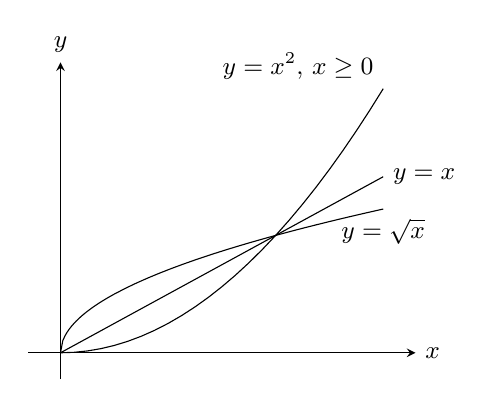
\begin{tikzpicture}[font=\small,declare function={f(\x)=\x^2;g(\x)=sqrt(\x);h(\x)=\x;}]
\begin{axis}[clip=false,small,axis lines=middle,enlargelimits=true,xlabel={$x$},ylabel={$y$},xlabel style={at={(current axis.right of origin)},anchor=west},ylabel style={at={(current axis.above origin)},anchor=south},xtick={\empty},ytick={\empty}]
\addplot[domain=0:1.5]{f(x)}node[above left]{$y=x^2,\, x\ge 0$};
\addplot[domain=0:0.25]{g(x)};
\addplot[domain=0.25:1.5]{g(x)}node[below]{$y=\sqrt{x}$};
\addplot[domain=0:1.5]{h(x)}node[right]{$y=x$};
\end{axis}
\end{tikzpicture}
\caption{
تفاعل \عددی{y=\sqrt{x}} اور \عددی{y=x^2,\, x\ge 0} ایک دوسرے کے الٹ ہیں (مثال \حوالہ{مثال_ماورائی_الٹ_تفاعل_کی_مثال})۔
}
\label{شکل_ماورائی_الٹ_تفاعل_تعریف}
\end{minipage}\hfill
\begin{minipage}{0.45\textwidth}
\centering
\begin{tikzpicture}[font=\small,declare function={f(\x)=1+3*(\x-1);g(\x)=\x;}]
\begin{axis}[clip=false,small,axis lines=middle,enlargelimits=true,xlabel={$x$},ylabel={$y$},xlabel style={at={(current axis.right of origin)},anchor=west},ylabel style={at={(current axis.above origin)},anchor=south},xtick={\empty},ytick={\empty}]
\addplot[domain=-0.25:2.25]{f(x)}node[above,align=left,xshift=3ex]{$y=\tfrac{1}{m}x-\tfrac{b}{m}$\\ ڈھلوان $\tfrac{1}{m}$};
\addplot[domain=0.25:3]({f(x)},x)node[pos=0.85,below,align=center,xshift=1ex]{$y=mx+b$\\ ڈھلوان m};
\addplot[domain=-0.5:5]{g(x)}node[right]{$y=x$};
\end{axis}
\end{tikzpicture}
\caption{
لکیر \عددی{y=x} میں منعکس غیر انتصابی لکیروں کے ڈھلوان ایک دوسرے کے بالعکس متناسب ہوتے ہیں۔
}
\label{شکل_ماورائی_عکس_میں_تفرق_تعلق}
\end{minipage}
\end{figure}


\جزوحصہء{قابل تفرق تفاعل کے الٹ کے تفرق}
تفاعل \عددی{f(x)=\tfrac{x}{2}+1}  اور اس کے الٹ \عددی{f^{-1}(x)=2x-2} (مثال \حوالہ{مثال_ماورائی_الٹ}) کے تفرق درج ذیل ہیں۔
\begin{align*}
\frac{\dif}{\dif x}f(x)&=\frac{\dif}{\dif x}\big(\frac{x}{2}+1\big)=\frac{1}{2}\\
\frac{\dif}{\dif x}f^{-1}(x)&=\frac{\dif}{\dif x}(2x-2)=2
\end{align*}
یہ تفرقات ایک دوسرے کے بالعکس متناسب ہیں۔ تفاعل \عددی{f} کی ترسیم لکیر \عددی{y=\tfrac{x}{2}+1} اور \عددی{f^{-1}} کی ترسیم لکیر \عددی{y=2x-2} ہے۔ ان لکیروں کے ڈھلوان ایک دوسرے کے بالعکس متناسب ہیں (شکل \حوالہ{شکل_ماورائی_عکس_میں_تفرق_تعلق})۔

یہ نتیجہ کسی مخصوص تفاعل کے لئے نہیں ہے۔ لکیر \عددی{y=x} میں کسی بھی غیر افقی یا غیر انتصابی لکیر کے عکس کا ڈھلوان اس لکیر کے ڈھلوان کے بالعکس متناسب ہو گا۔ یوں اگر دیے گئے لکیر کا ڈھلوان \عددی{m\ne 0} (شکل \حوالہ{شکل_ماورائی_عکس_میں_تفرق_تعلق}) ہو تب منعکس لکیر کا ڈھلوان \عددی{\tfrac{1}{m}} ہو گا۔ 

تفاعل اور اس کے الٹ کے ڈھلوانوں  کا بالعکس متناسب تعلق دیگر تفاعل کو بھی مطمئن کرتا ہے۔ اگر نقطہ \عددی{(a,f(a))} پر \عددی{y=f(x)} کا ڈھلوان \عددی{f'(a)\ne 0} ہو تب مطابقتی نقطہ \عددی{(f(a),a)} پر \عددی{y=f^{-1}(x)} کا ڈھلوان \عددی{\tfrac{1}{f'(a)}} ہو گا (شکل \حوالہ{شکل_ماورائی_ڈھلوان_بالعکس_متناسب})۔ یوں نقطہ \عددی{f(a)} پر \عددی{f^{-1}} کا تفرق، نقطہ \عددی{a} پر \عددی{f} کے تفرق کا بالعکس متناسب ہو گا۔ یہ تعلق اس صورت درست ہو گا جب \عددی{f} درج ذیل مسئلہ میں پیش   شرائط کو مطمئن کرتا ہو۔ یہ شرائط اعلٰی احصاء سے حاصل ہوتے ہیں۔ 

\begin{figure}
\centering
\begin{subfigure}{0.45\textwidth}
\centering
\begin{tikzpicture}[font=\small,declare function={f(\x)=(\x-1)^2;g(\x)=1+sqrt(\x);ta(\x)=9/16+3/2*(\x-7/4);}]
\pgfmathsetmacro{\a}{1.75}
\pgfmathsetmacro{\b}{f(\a)}
\begin{axis}[clip=false,small,axis lines=middle,enlargelimits=true,xlabel={$x$},ylabel={$y$},xlabel style={at={(current axis.right of origin)},anchor=west},ylabel style={at={(current axis.above origin)},anchor=south},xtick={\a}, xticklabels={$a$}, ytick={\b}, yticklabels={$f(a)$}]
\addplot[domain=1:2.2]{f(x)}node[above left]{$y=f(x)$};
%\addplot[domain=0:0.5]{g(x)};
%\addplot[domain=0.5:1.5]{g(x)};
\draw(\a,\b)node[circ]{}node[right,yshift=-1ex]{$(a,f(a))$};
%\draw(\b,\a)node[circ]{};
\addplot[domain=1.25:2.2]{ta(x)};
%\addplot[domain=1.25:2.25]({ta(x)},x);
\end{axis}
\end{tikzpicture}
\end{subfigure}\hfill
\begin{subfigure}{0.45\textwidth}
\centering
\begin{tikzpicture}[font=\small,declare function={f(\x)=(\x-1)^2;g(\x)=1+sqrt(\x);ta(\x)=9/16+3/2*(\x-7/4);}]
\pgfmathsetmacro{\a}{1.75}
\pgfmathsetmacro{\b}{f(\a)}
\begin{axis}[clip=false,small,axis lines=middle,enlargelimits=true,xlabel={$x$},ylabel={$y$},xlabel style={at={(current axis.right of origin)},anchor=west},ylabel style={at={(current axis.above origin)},anchor=south},xtick={\b},xticklabels={$f(a)$},ytick={\a},yticklabels={$a$}]
%\addplot[domain=1:2.2]{f(x)};
\addplot[domain=0:0.5]{g(x)};
\addplot[domain=0.5:1.5]{g(x)}node[pos=0.75,below right]{$y=f^{-1}(x)$};
%\draw(\a,\b)node[circ]{};
\draw(\b,\a)node[circ]{}node[right,yshift=-1ex]{$(f(a),a)$};
%\addplot[domain=1:2.2]{ta(x)};
\addplot[domain=1.4:2.25]({ta(x)},x);
\end{axis}
\end{tikzpicture}
\end{subfigure}
\caption{
الٹ تفاعل کے مطابقتی نقطوں پر ڈھلوان ایک دوسرے کا بالعکس متناسب 
\عددی{\left.\tfrac{\dif f^{-1}}{\dif x}\right\vert_{f(a)}=\tfrac{1}{\left.\tfrac{\dif f}{\dif x}\right\vert_{a}}} ہو گا۔
}
\label{شکل_ماورائی_ڈھلوان_بالعکس_متناسب}
\end{figure}
\ابتدا{مسئلہ}\شناخت{مسئلہ_ماورائی_الٹ_تفرق_قاعدہ}\موٹا{الٹ تفاعل کے تفرق کا قاعدہ}\\
اگر وقفہ \عددی{I} کے ہر نقطہ پر \عددی{f} قابل تفرق ہو اور \عددی{I} پر \عددی{\tfrac{\dif f}{\dif x}} کبھی بھی صفر  نہ ہو، تب وقفہ \عددی{f(I)} کے ہر نقطہ پر \عددی{f^{-1}} قابل تفرق ہو گا۔ کسی ایک مخصوص نقطہ \عددی{f(a)} پر \عددی{\tfrac{\dif f^{-1}}{\dif x}} کا تفرق نقطہ \عددی{a} پر تفرق \عددی{\tfrac{\dif f}{\dif x}} کا بالعکس متناسب ہو گا:
\begin{align}\label{مساوات_ماورائی_قاعدہ_الٹ_تفرق_الف}
\big(\frac{\dif f^{-1}}{\dif x}\big)_{x=f(a)}=\frac{1}{\big(\frac{\dif f}{\dif x}\big)_{x=a}}
\end{align}
اس کو مختصراً درج ذیل لکھا جا سکتا ہے۔
\begin{align}\label{مساوات_ماورائی_قاعدہ_الٹ_تفرق_ب}
(f^{-1})'=\frac{1}{f'}
\end{align}
\انتہا{مسئلہ}
%==================

\ابتدا{مثال}\شناخت{مثال_ماورائی_تفرق_الٹ_تفرق}
تفاعل \عددی{f(x)=x^2,\,x\ge 0} اور اس کے الٹ \عددی{f^{-1}(x)=\sqrt{x}} کے لئے درج ذیل لکھا جا سکتا ہے۔
\begin{align*}
\frac{\dif f}{\dif x}=\frac{\dif}{\dif x}(x^2)=2x,\quad \frac{\dif f^{-1}}{\dif x}=\frac{\dif}{\dif x}\sqrt{x}=\frac{1}{2\sqrt{x}},\,\,x>0
\end{align*}
نقطہ \عددی{(4,2)} لکیر \عددی{y=x} کی دوسری طرف نقطہ \عددی{(2,4)} کا عکس ہے (شکل \حوالہ{شکل_مثال_ماورائی_تفرق_الٹ_تفرق})۔ان نقطوں پر درج ذیل حاصل ہو گا۔
\begin{align*}
\frac{\dif f}{\dif x}&=2x=2(2)=4&&\text{\RL{نقطہ $(2,4)$ پر}}\\
\frac{\dif f^{-1}}{\dif x}&=\frac{1}{2\sqrt{x}}=\frac{1}{2\sqrt{4}}=\frac{1}{4}=\frac{1}{\dif f/\dif x}&&\text{\RL{نقطہ $(4,2)$ پر}}
\end{align*}
\انتہا{مثال}
%====================
\begin{figure}
\centering
\begin{minipage}{0.45\textwidth}
\centering
\begin{tikzpicture}[font=\small,declare function={f(\x)=\x^2;ta(\x)=4+4*(\x-2);tb(\x)=2+1/4*(\x-4);}]
\begin{axis}[clip=false,small,axis lines=middle,enlargelimits=true,xlabel={$x$},ylabel={$y$},xlabel style={at={(current axis.right of origin)},anchor=west},ylabel style={at={(current axis.above origin)},anchor=south},xtick={2,4},ytick={2,4}]
\addplot[domain=0:2.5]{f(x)}node[above,xshift=3ex]{$y=x^2,\, x \ge 0$};
\addplot[domain=0:3]({f(x)},{x})node[below]{$y=\tfrac{1}{\sqrt{x}}$};
\addplot[thick,domain=1.5:2.5]{ta(x)};
\addplot[thick,domain=2.5:8]{tb(x)};
\draw(2,4)node[circ]{}node[left]{$(2,4)$}node[right]{ڈھلوان 4};
\draw(4,2)node[circ]{}node[below]{$(4,2)$}node[above]{ڈھلوان $\tfrac{1}{4}$};
\end{axis}
\end{tikzpicture}
\caption{
نقطہ \عددی{(4,2)} پر \عددی{f^{-1}(x)=\sqrt{x}} کا تفرق نقطہ \عددی{(2,4)} پر \عددی{f(x)=x^2} کے تفرق کا بالعکس متناسب ہو گا (مثال \حوالہ{مثال_ماورائی_تفرق_الٹ_تفرق})۔
}
\label{شکل_مثال_ماورائی_تفرق_الٹ_تفرق}
\end{minipage}\hfill
\begin{minipage}{0.45\textwidth}
\centering
\begin{tikzpicture}[font=\small,declare function={f(\x)=\x^3-2;g(\x)=(\x+2)^(1/3); ta(\x)=6+12*(\x-2);tb(\x)=2+1/12*(\x-6);}]
\begin{axis}[clip=false,small,axis lines=middle,enlargelimits=true,xlabel={$x$},ylabel={$y$},xlabel style={at={(current axis.right of origin)},anchor=west},ylabel style={at={(current axis.above origin)},anchor=south},xtick={-2,6},ytick={-2,6}]
\addplot[domain=0:2.05]{f(x)}node[above,xshift=3ex]{$y=x^3-2$};
\addplot[domain=-2:-1.5]{g(x)};
\addplot[domain=-1.5:7]{g(x)};
\addplot[thick,domain=1.75:2.05]{ta(x)};
\addplot[thick,domain=3:7]{tb(x)};
\draw(2,6)node[circ]{}node[left]{$(2,6)$}node[right]{ڈھلوان 12};
\draw(6,2)node[circ]{}node[below]{$(6,2)$}node[above]{الٹ ڈھلوان $\tfrac{1}{12}$};
\end{axis}
\end{tikzpicture}
\caption{
نقطہ \عددی{x=2} پر \عددی{f(x)=x^3-2} کا تفرق ہمیں نقطہ \عددی{x=6} پر \عددی{f^{-1}} کا تفرق دیتا  ہے (مثال \حوالہ{مثال_ماورائی_ایک_نقطہ_پر_تفرق_سے_الٹ_تفرق_کا_حصول})۔
}
\label{شکل_مثال_ماورائی_ایک_نقطہ_پر_تفرق_سے_الٹ_تفرق_کا_حصول}
\end{minipage}
\end{figure}

بعض اوقات \عددی{f^{-1}} کا کلیہ نہ جانتے ہوئے بھی مساوات \حوالہ{مساوات_ماورائی_قاعدہ_الٹ_تفرق_الف} کی مدد سے \عددی{\tfrac{\dif f^{-1}}{\dif x}} کی مخصوص قیمتیں تلاش کی جا سکتی ہیں۔

\ابتدا{مثال}\شناخت{مثال_ماورائی_ایک_نقطہ_پر_تفرق_سے_الٹ_تفرق_کا_حصول}
مان لیں \عددی{f(x)=x^3-2} ہے۔ \عددی{f^{-1}(x)} کا کلیہ دریافت کیے بغیر نقطہ \عددی{x=6=f(2)} پر \عددی{\tfrac{\dif f^{-1}}{\dif x}} کی قیمت تلاش کریں۔

حل:  (شکل \حوالہ{شکل_مثال_ماورائی_ایک_نقطہ_پر_تفرق_سے_الٹ_تفرق_کا_حصول})
\begin{align*}
\left.\frac{\dif f}{\dif x}\right\vert_{x=2}&=\left.3x^2\right\vert_{x=2}=12\\
\left.\frac{\dif f^{-1}}{\dif x}\right\vert_{x=f(2)}&=\frac{1}{12}&&\text{\RL{مساوات \حوالہ{مساوات_ماورائی_قاعدہ_الٹ_تفرق_الف}}}
\end{align*}
\انتہا{مثال}
%=======================

مسئلہ \حوالہ{مسئلہ_ماورائی_الٹ_تفرق_قاعدہ} کو ایک مختلف نقطہ نظر سے دیکھا جا سکتا ہے۔ اگر \عددی{x=a} پر \عددی{y=f(x)}  قابل تفرق ہو اور ہم \عددی{x} کی قیمت میں معمولی تبدیلی \عددی{\dif x} لائیں تب \عددی{y} میں مطابقتی تبدیلی تخمیناً
\begin{align*}
\dif y=f'(a)\dif x
\end{align*}
ہو گا۔اس کا مطلب ہے کہ \عددی{y} کی تبدیلی، \عددی{x} کی تبدیلی کے تقریباً \عددی{f'(a)} گنّا ہو گی اور \عددی{x} کی تبدیلی، \عددی{y} کی تبدیلی کے تقریباً  \عددی{\tfrac{1}{f'(a)}} گنّا ہو گی۔

\حصہء{سوالات}
\موٹا{ایک ایک تفاعل کی نشاندہی}\\
سوال \حوالہ{سوال_ماورائی_ایک_ایک_نشاندہی_الف} تا سوال \حوالہ{سوال_ماورائی_ایک_ایک_نشاندہی_ث} میں تفاعل کے ترسیم دیے گئے ہیں۔ ان میں  ایک ایک تفاعل کی نشاندہی کریں۔

\ابتدا{سوال}\شناخت{سوال_ماورائی_ایک_ایک_نشاندہی_الف}
ترسیم شکل \حوالہ{شکل_سوال_ماورائی_ایک_ایک_نشاندہی_الف} میں دی گئی ہے۔
\انتہا{سوال}
%=======================
\ابتدا{سوال}\شناخت{سوال_ماورائی_ایک_ایک_نشاندہی_ب}
ترسیم شکل \حوالہ{شکل_سوال_ماورائی_ایک_ایک_نشاندہی_ب} میں دی گئی ہے۔
\انتہا{سوال}
%=======================
\ابتدا{سوال}\شناخت{سوال_ماورائی_ایک_ایک_نشاندہی_پ}
ترسیم شکل \حوالہ{شکل_سوال_ماورائی_ایک_ایک_نشاندہی_پ} میں دی گئی ہے۔
\انتہا{سوال}
%=======================
\ابتدا{سوال}\شناخت{سوال_ماورائی_ایک_ایک_نشاندہی_ت}
ترسیم شکل \حوالہ{شکل_سوال_ماورائی_ایک_ایک_نشاندہی_ت} میں دی گئی ہے۔
\انتہا{سوال}
%=======================
\ابتدا{سوال}\شناخت{سوال_ماورائی_ایک_ایک_نشاندہی_ٹ}
ترسیم شکل \حوالہ{شکل_سوال_ماورائی_ایک_ایک_نشاندہی_ٹ} میں دی گئی ہے۔
\انتہا{سوال}
%=======================
\ابتدا{سوال}\شناخت{سوال_ماورائی_ایک_ایک_نشاندہی_ث}
ترسیم شکل \حوالہ{شکل_سوال_ماورائی_ایک_ایک_نشاندہی_ث} میں دی گئی ہے۔
\انتہا{سوال}
%=================
\begin{figure}
\centering
\begin{minipage}{0.3\textwidth}
\centering
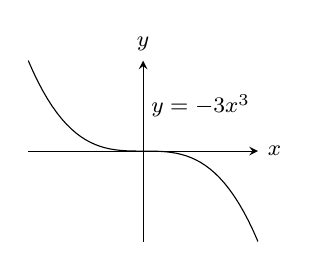
\begin{tikzpicture}[font=\footnotesize,declare function={f(\x)=-3*\x^3;}]
\begin{axis}[width=4.5cm,axis lines=middle,xlabel={$x$},ylabel={$y$},xlabel style={at={(current axis.right of origin)},anchor=west},ylabel style={at={(current axis.above origin)},anchor=south},xtick={\empty},ytick={\empty}]
\addplot[domain=0:2]{f(x)};
\addplot[domain=0:2]({-x},{-f(x)});
\draw(1,{-1/2*f(2)})node[]{$y=-3x^3$};
\end{axis}
\end{tikzpicture}
\caption{ترسیم برائے سوال \حوالہ{سوال_ماورائی_ایک_ایک_نشاندہی_الف}}
\label{شکل_سوال_ماورائی_ایک_ایک_نشاندہی_الف}
\end{minipage}\hfill
\begin{minipage}{0.3\textwidth}
\centering
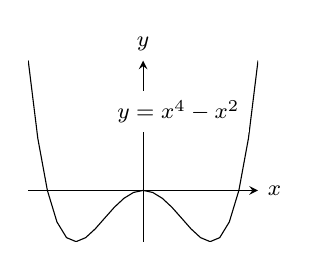
\begin{tikzpicture}[font=\footnotesize,declare function={f(\x)=\x^4-\x^2;}]
\begin{axis}[width=4.5cm,axis lines=middle,xlabel={$x$},ylabel={$y$},xlabel style={at={(current axis.right of origin)},anchor=west},ylabel style={at={(current axis.above origin)},anchor=south},xtick={\empty},ytick={\empty}]
\addplot[domain=-1.2:1.2]{f(x)}node[pos=0.9,above left,fill=white]{$y=x^4-x^2$};
\end{axis}
\end{tikzpicture}
\caption{ترسیم برائے سوال \حوالہ{سوال_ماورائی_ایک_ایک_نشاندہی_ب}}
\label{شکل_سوال_ماورائی_ایک_ایک_نشاندہی_ب}
\end{minipage}\hfill
\begin{minipage}{0.3\textwidth}
\centering
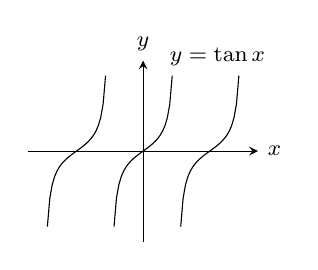
\begin{tikzpicture}[font=\footnotesize,declare function={f(\x)=tan(deg(\x));}]
\begin{axis}[clip=false,width=4.5cm,axis lines=middle,xlabel={$x$},ylabel={$y$},xlabel style={at={(current axis.right of origin)},anchor=west},ylabel style={at={(current axis.above origin)},anchor=south},xtick={\empty},ytick={\empty},enlargelimits=true]
\addplot[domain=-3/2*pi+0.2:-pi/2-0.2]{f(x)};
\addplot[domain=-pi/2+0.2:pi/2-0.2]{f(x)};
\addplot[domain=pi/2+0.2:3/2*pi-0.2]{f(x)}node[above  left,xshift=3ex]{$y=\tan x$};
\end{axis}
\end{tikzpicture}
\caption{ترسیم برائے سوال \حوالہ{سوال_ماورائی_ایک_ایک_نشاندہی_پ}}
\label{شکل_سوال_ماورائی_ایک_ایک_نشاندہی_پ}
\end{minipage}
\end{figure}
%======================
\begin{figure}
\centering
\begin{minipage}{0.3\textwidth}
\centering
\begin{tikzpicture}[font=\footnotesize,declare function={f(\x)=-3*\x^3;}]
\pgfmathsetmacro{\k}{1.25/5}
\draw[-latex](-1.25,0)--(1.25,0)node[right]{$x$};
\draw[-latex](0,-1.25)--(0,1.25)node[above]{$y$};
\foreach \x in {-1,-2,-3,-4,0,1,2,3}{\draw(\x*\k,\x*\k)node[circ]{}--++(\k,0)node[ocirc]{};}
\draw(-0.75,0.75)node[]{$y=\lfloor x\rfloor$};
\end{tikzpicture}
\caption{ترسیم برائے سوال \حوالہ{سوال_ماورائی_ایک_ایک_نشاندہی_ت}}
\label{شکل_سوال_ماورائی_ایک_ایک_نشاندہی_ت}
\end{minipage}\hfill
\begin{minipage}{0.3\textwidth}
\centering
\begin{tikzpicture}[font=\footnotesize,declare function={f(\x)=1/\x;}]
\begin{axis}[width=4.5cm,axis lines=middle,xlabel={$x$},ylabel={$y$},xlabel style={at={(current axis.right of origin)},anchor=west},ylabel style={at={(current axis.above origin)},anchor=south},xtick={\empty},ytick={\empty}]
\addplot[domain=0.2:5]{f(x)}node[pos=0.25,right]{$y=\tfrac{1}{x}$};
\addplot[domain=0.2:5](-x,{-f(x)});
\end{axis}
\end{tikzpicture}
\caption{ترسیم برائے سوال \حوالہ{سوال_ماورائی_ایک_ایک_نشاندہی_ٹ}}
\label{شکل_سوال_ماورائی_ایک_ایک_نشاندہی_ٹ}
\end{minipage}\hfill
\begin{minipage}{0.3\textwidth}
\centering
\begin{tikzpicture}[font=\footnotesize,declare function={f(\x)=\x^(1/3);}]
\begin{axis}[clip=false,width=4.5cm,axis lines=middle,xlabel={$x$},ylabel={$y$},xlabel style={at={(current axis.right of origin)},anchor=west},ylabel style={at={(current axis.above origin)},anchor=south},xtick={\empty},ytick={\empty},enlargelimits=true]
\addplot[domain=0:6]{f(x)};
\draw (-3,1)node[]{$y=x^{1/3}$};
\addplot[domain=0:6](-x,{-f(x)});
\end{axis}
\end{tikzpicture}
\caption{ترسیم برائے سوال \حوالہ{سوال_ماورائی_ایک_ایک_نشاندہی_ث}}
\label{شکل_سوال_ماورائی_ایک_ایک_نشاندہی_ث}
\end{minipage}
\end{figure}

\موٹا{الٹ تفاعل کی ترسیم}\\
سوال \حوالہ{سوال_ماورائی_ترسیم_دیا_الف} تا سوال \حوالہ{سوال_ماورائی_ترسیم_دیا_ت} میں \عددی{y=f(x)} کی ترسیم دی گئی ہے۔ اس کو نقل کر کے لکیر  \عددی{y=x} بھی بنائیں۔ لکیر \عددی{y=x} کے لحاظ سے تشاکلی استعمال کرتے ہوئے \عددی{y=f^{-1}(x)} ترسیم کریں۔(\عددی{f^{-1}} کا کلیہ معلوم کرنے کی ضرورت نہیں ہے۔) \عددی{f^{-1}} کے دائرہ کار اور سعت کی نشاندہی  کریں۔

\ابتدا{سوال}\شناخت{سوال_ماورائی_ترسیم_دیا_الف}
تفاعل کی ترسیم شکل \حوالہ{شکل_سوال_ماورائی_ترسیم_دیا_الف} میں دی گئی ہے۔
\انتہا{سوال}
%=======================
\ابتدا{سوال}\شناخت{سوال_ماورائی_ترسیم_دیا_ب}
تفاعل کی ترسیم شکل \حوالہ{شکل_سوال_ماورائی_ترسیم_دیا_ب} میں دی گئی ہے۔
\انتہا{سوال}
%=======================
\ابتدا{سوال}\شناخت{سوال_ماورائی_ترسیم_دیا_پ}
تفاعل کی ترسیم شکل \حوالہ{شکل_سوال_ماورائی_ترسیم_دیا_پ} میں دی گئی ہے۔
\انتہا{سوال}
%=======================
\ابتدا{سوال}\شناخت{سوال_ماورائی_ترسیم_دیا_ت}
تفاعل کی ترسیم شکل \حوالہ{شکل_سوال_ماورائی_ترسیم_دیا_ت} میں دی گئی ہے۔
\انتہا{سوال}
%=======================
\begin{figure}
\centering
\begin{minipage}{0.2\textwidth}
\centering
\begin{tikzpicture}[font=\tiny,declare function={f(\x)=1/(\x^2+1);}]
\begin{axis}[clip=false,width=4cm,axis lines=middle,xlabel={$x$},ylabel={$y$},xlabel style={at={(current axis.right of origin)},anchor=west},ylabel style={at={(current axis.above origin)},anchor=south},xtick={1},ytick={1},enlargelimits=true,ymin=0]
\addplot[domain=0:2]{f(x)}node[pos=0.5,above right]{$\begin{aligned}y&=f(x)\\ &=\frac{1}{\x^2+1},\, x\ge 0\end{aligned}$};
\end{axis}
\end{tikzpicture}
\caption{ترسیم برائے سوال \حوالہ{سوال_ماورائی_ترسیم_دیا_الف}}
\label{شکل_سوال_ماورائی_ترسیم_دیا_الف}
\end{minipage}\hfill
\begin{minipage}{0.2\textwidth}
\centering
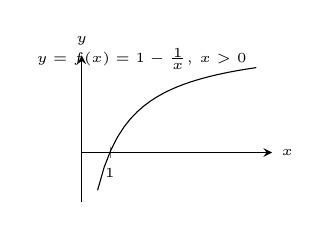
\begin{tikzpicture}[font=\tiny,declare function={f(\x)=1-1/\x;}]
\begin{axis}[clip=false,width=4cm,axis lines=middle,xlabel={$x$},ylabel={$y$},xlabel style={at={(current axis.right of origin)},anchor=west},ylabel style={at={(current axis.above origin)},anchor=south},xtick={1},ytick={1},enlargelimits=true]
\addplot[domain=0.75:4]{f(x)}node[pos=1,above left,yshift=-1ex]{$y=f(x)=1-\frac{1}{x},\, x> 0$};
\end{axis}
\end{tikzpicture}
\caption{ترسیم برائے سوال \حوالہ{سوال_ماورائی_ترسیم_دیا_ب}}
\label{شکل_سوال_ماورائی_ترسیم_دیا_ب}
\end{minipage}\hfill
\begin{minipage}{0.2\textwidth}
\centering
\begin{tikzpicture}[font=\tiny,declare function={f(\x)=sin(deg(\x));}]
\pgfmathsetmacro{\k}{1/2*pi}
\begin{axis}[clip=false,width=4cm,axis lines=middle,xlabel={$x$},ylabel={$y$},xlabel style={at={(current axis.right of origin)},anchor=west},ylabel style={at={(current axis.above origin)},anchor=south},xtick={-\k,\k},xticklabels={$-\tfrac{\pi}{2}$,$\tfrac{\pi}{2}$},ytick={-1,1},enlargelimits=true]
\addplot[domain=-1/2*pi:1/2*pi]{f(x)};
\draw(-1/2*pi,1)node[]{$\begin{aligned}y&=f(x)=\sin x\\  &-\tfrac{\pi}{2}\le x\le \tfrac{\pi}{2}\end{aligned}$};
\draw(-\k,-1)node[circ]{}  (\k,1)node[circ]{};
\end{axis}
\end{tikzpicture}
\caption{ترسیم برائے سوال \حوالہ{سوال_ماورائی_ترسیم_دیا_پ}}
\label{شکل_سوال_ماورائی_ترسیم_دیا_پ}
\end{minipage}\hfill
\begin{minipage}{0.2\textwidth}
\centering
\begin{tikzpicture}[font=\tiny,declare function={f(\x)=tan(deg(\x));}]
\pgfmathsetmacro{\k}{1/2*pi}
\begin{axis}[clip=false,width=4cm,axis lines=middle,xlabel={$x$},ylabel={$y$},xlabel style={at={(current axis.right of origin)},anchor=west},ylabel style={at={(current axis.above origin)},anchor=south}, xtick={-\k,\k},  xticklabels={$-\tfrac{\pi}{2}$,$\tfrac{\pi}{2}$}, ytick={\empty},enlargelimits=true]
\addplot[domain=-\k+0.4:\k-0.4]{f(x)};
\draw(-1/2*pi,2)node[]{$\begin{aligned}y&=f(x)=\tan x\\  &-\tfrac{\pi}{2}< x<\tfrac{\pi}{2}\end{aligned}$};
\end{axis}
\end{tikzpicture}
\caption{ترسیم برائے سوال \حوالہ{سوال_ماورائی_ترسیم_دیا_ت}}
\label{شکل_سوال_ماورائی_ترسیم_دیا_ت}
\end{minipage}
\end{figure}

\ابتدا{سوال}
(ا) تفاعل \عددی{f(x)=\sqrt{1-x^2},\, 0\le x\le 1} ترسیم کریں۔ اس ترسیم میں کون سی تشاکلی پائی جاتی ہے؟ (ب) دکھائیں کہ \عددی{f} اپنا ہی الٹ ہے۔ (یاد رہے کہ \عددی{x\ge 0} کی صورت میں \عددی{\sqrt{x^2}=x} ہوتا ہے۔)
\انتہا{سوال}
%==============
\ابتدا{سوال}
(ا) تفاعل \عددی{f(x)=\tfrac{1}{x}} ترسیم کریں۔ اس ترسیم میں کون سی تشاکلی پائی جاتی ہے؟ (ب) دکھائیں کہ \عددی{f} اپنا ہی الٹ ہے۔
\انتہا{سوال}
%==================
\موٹا{الٹ تفاعل کے کلیات}\\
سوال \حوالہ{سوال_ماورائی_ترسیم_کلیہ_الف} تا سوال \حوالہ{سوال_ماورائی_ترسیم_کلیہ_ث} میں تفاعل \عددی{y=f(x)} کا کلیہ دیا گیا ہے۔ \عددی{f} اور \عددی{f^{-1}} کی ترسیمات بھی دکھائی گئی ہیں۔ \عددی{f^{-1}} کا کلیہ تلاش کریں۔

\ابتدا{سوال}\شناخت{سوال_ماورائی_ترسیم_کلیہ_الف}
$f(x)=x^2+1,\quad x\ge 0$
ترسیم شکل \حوالہ{شکل_سوال_ماورائی_ترسیم_کلیہ_الف} میں دی گئی ہے۔
\انتہا{سوال}
%===================
\ابتدا{سوال}\شناخت{سوال_ماورائی_ترسیم_کلیہ_ب}
$f(x)=x^2,\quad x\le 0$
ترسیم شکل \حوالہ{شکل_سوال_ماورائی_ترسیم_کلیہ_ب} میں دی گئی ہے۔
\انتہا{سوال}
%===================
\ابتدا{سوال}\شناخت{سوال_ماورائی_ترسیم_کلیہ_پ}
$f(x)=x^3-1$
ترسیم شکل \حوالہ{شکل_سوال_ماورائی_ترسیم_کلیہ_پ} میں دی گئی ہے۔
\انتہا{سوال}
%===================
\ابتدا{سوال}\شناخت{سوال_ماورائی_ترسیم_کلیہ_ت}
$f(x)=x^2-2x+1,\quad x\ge 1$
ترسیم شکل \حوالہ{شکل_سوال_ماورائی_ترسیم_کلیہ_ت} میں دی گئی ہے۔
\انتہا{سوال}
%===================
\ابتدا{سوال}\شناخت{سوال_ماورائی_ترسیم_کلیہ_ٹ}
$f(x)=(x+1)^2,\quad x\ge -1$
ترسیم شکل \حوالہ{شکل_سوال_ماورائی_ترسیم_کلیہ_ٹ} میں دی گئی ہے۔
\انتہا{سوال}
%===================
\ابتدا{سوال}\شناخت{سوال_ماورائی_ترسیم_کلیہ_ث}
$f(x)=x^{2/3},\quad x\ge 0$
ترسیم شکل \حوالہ{شکل_سوال_ماورائی_ترسیم_کلیہ_ث} میں دی گئی ہے۔
\انتہا{سوال}
%===================
\begin{figure}
\centering
\begin{minipage}{0.3\textwidth}
\centering
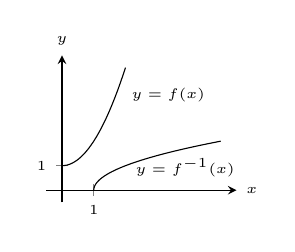
\begin{tikzpicture}[font=\tiny,declare function={f(\x)=\x^2+1;}]
\begin{axis}[clip=false,width=4cm,axis lines=middle,xlabel={$x$},ylabel={$y$},xlabel style={at={(current axis.right of origin)},anchor=west},ylabel style={at={(current axis.above origin)},anchor=south},xtick={1},ytick={1},enlargelimits=true,ymin=0]
\addplot[domain=0:2]{f(x)}node[pos=0.9,below right]{$y=f(x)$};
\addplot[domain=0:2]({f(x)},x)node[pos=0.75,below]{$y=f^{-1}(x)$};
\end{axis}
\end{tikzpicture}
\caption{ترسیم برائے سوال \حوالہ{سوال_ماورائی_ترسیم_کلیہ_الف}}
\label{شکل_سوال_ماورائی_ترسیم_کلیہ_الف}
\end{minipage}\hfill
\begin{minipage}{0.3\textwidth}
\centering
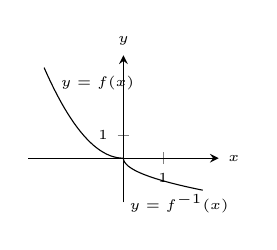
\begin{tikzpicture}[font=\tiny,declare function={f(\x)=\x^2;}]
\begin{axis}[clip=false,width=4cm,axis lines=middle,xlabel={$x$},ylabel={$y$},xlabel style={at={(current axis.right of origin)},anchor=west},ylabel style={at={(current axis.above origin)},anchor=south},xtick={1},ytick={1},enlargelimits=true]
\addplot[domain=0:2](-x,{f(x)})node[pos=0.85,right]{$y=f(x)$};
\addplot[domain=0:1.4142]({f(x)},-x)node[pos=0.75,below]{$y=f^{-1}(x)$};
\end{axis}
\end{tikzpicture}
\caption{ترسیم برائے سوال \حوالہ{سوال_ماورائی_ترسیم_کلیہ_ب}}
\label{شکل_سوال_ماورائی_ترسیم_کلیہ_ب}
\end{minipage}\hfill
\begin{minipage}{0.3\textwidth}
\centering
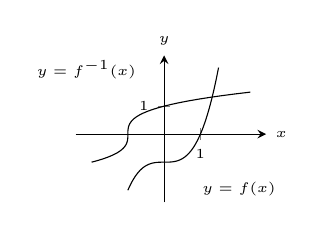
\begin{tikzpicture}[font=\tiny,declare function={f(\x)=\x^3-1;g(\x)=\x^3+1;}]
\begin{axis}[clip=false,width=4cm,axis lines=middle,xlabel={$x$},ylabel={$y$},xlabel style={at={(current axis.right of origin)},anchor=west},ylabel style={at={(current axis.above origin)},anchor=south},xtick={1},ytick={1},enlargelimits=true]
\addplot[domain=0:1.5]{f(x)}node[pos=0.25,below right,yshift={-2ex}]{$y=f(x)$};
\addplot[domain=0:1](-x,{-g(x)});
\addplot[domain=0:1.5]({f(x)},x)node[pos=0.25,above left,yshift=2ex]{$y=f^{-1}(x)$};
\addplot[domain=0:1]({-g(x)},-x);
\end{axis}
\end{tikzpicture}
\caption{ترسیم برائے سوال \حوالہ{سوال_ماورائی_ترسیم_کلیہ_پ}}
\label{شکل_سوال_ماورائی_ترسیم_کلیہ_پ}
\end{minipage}
\end{figure}
%==============================
\begin{figure}
\centering
\begin{minipage}{0.3\textwidth}
\centering
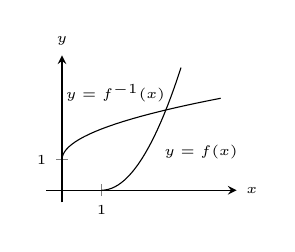
\begin{tikzpicture}[font=\tiny,declare function={f(\x)=\x^2-2*\x+1;}]
\begin{axis}[clip=false,width=4cm,axis lines=middle,xlabel={$x$},ylabel={$y$},xlabel style={at={(current axis.right of origin)},anchor=west},ylabel style={at={(current axis.above origin)},anchor=south},xtick={1},ytick={1},enlargelimits=true,ymin=0]
\addplot[domain=1:3]{f(x)}node[pos=0.5,below right]{$y=f(x)$};
\addplot[domain=1:3]({f(x)},x)node[pos=0.4,above,yshift=1ex]{$y=f^{-1}(x)$};
\end{axis}
\end{tikzpicture}
\caption{ترسیم برائے سوال \حوالہ{سوال_ماورائی_ترسیم_کلیہ_ت}}
\label{شکل_سوال_ماورائی_ترسیم_کلیہ_ت}
\end{minipage}\hfill
\begin{minipage}{0.3\textwidth}
\centering
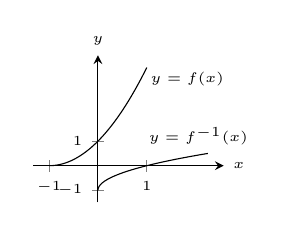
\begin{tikzpicture}[font=\tiny,declare function={f(\x)=(\x+1)^2;g(\x)=(\x-1)^2;}]
\begin{axis}[clip=false,width=4cm,axis lines=middle,xlabel={$x$},ylabel={$y$},xlabel style={at={(current axis.right of origin)},anchor=west},ylabel style={at={(current axis.above origin)},anchor=south},xtick={-1,1},ytick={-1,1},enlargelimits=true]
\addplot[domain=0:1](x,{f(x)})node[pos=0.85,right]{$y=f(x)$};
\addplot[domain=0:1](-x,{g(x)});
\addplot[domain=0:0.5]({f(x)},x)node[pos=0.85,above]{$y=f^{-1}(x)$};
\addplot[domain=0:1]({g(x)},-x);
\end{axis}
\end{tikzpicture}
\caption{ترسیم برائے سوال \حوالہ{سوال_ماورائی_ترسیم_کلیہ_ٹ}}
\label{شکل_سوال_ماورائی_ترسیم_کلیہ_ٹ}
\end{minipage}\hfill
\begin{minipage}{0.3\textwidth}
\centering
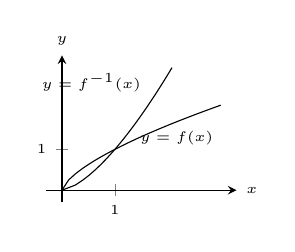
\begin{tikzpicture}[font=\tiny,declare function={f(\x)=(\x^2)^(1/3);}]
\begin{axis}[clip=false,width=4cm,axis lines=middle,xlabel={$x$},ylabel={$y$},xlabel style={at={(current axis.right of origin)},anchor=west},ylabel style={at={(current axis.above origin)},anchor=south},xtick={1},ytick={1},enlargelimits=true]
\addplot[domain=0:3]{f(x)}node[pos=0.75,below]{$y=f(x)$};
\addplot[domain=0:3]({f(x)},x)node[pos=0.75,above left,]{$y=f^{-1}(x)$};
\end{axis}
\end{tikzpicture}
\caption{ترسیم برائے سوال \حوالہ{سوال_ماورائی_ترسیم_کلیہ_ث}}
\label{شکل_سوال_ماورائی_ترسیم_کلیہ_ث}
\end{minipage}
\end{figure}

سوال \حوالہ{سوال_ماورائی_تصدیق_الف} تا سوال \حوالہ{سوال_ماورائی_تصدیق_ب} میں تفاعل \عددی{y=f(x)} کا کلیہ دیا گیا ہے۔ \عددی{f^{-1}} دریافت کریں اور اس کے دائرہ کار اور سعت کی نشاندہی کریں۔ تصدیق کی خاطر دکھائیں کہ \عددی{f(f^{-1}(x))=f^{-1}(f(x))=x} ہے۔ 

\ابتدا{سوال}\شناخت{سوال_ماورائی_تصدیق_الف}
$f(x)=x^5$
\انتہا{سوال}
%======================
\ابتدا{سوال}
$f(x)=x^4,\quad x\ge 0$
\انتہا{سوال}
%======================
\ابتدا{سوال}
$f(x)=x^3+1$
\انتہا{سوال}
%======================
\ابتدا{سوال}
$f(x)=\tfrac{x}{2}-\tfrac{7}{2}$
\انتہا{سوال}
%======================
\ابتدا{سوال}
$f(x)=\tfrac{1}{x^2},\quad x>0$
\انتہا{سوال}
%======================
\ابتدا{سوال}\شناخت{سوال_ماورائی_تصدیق_ب}
$f(x)=\tfrac{1}{x^3},\quad x\ne 0$
\انتہا{سوال}
%======================
